\documentclass[a4paper, 11pt]{report}
\usepackage[top=2.5cm, bottom=2.5cm, left=2cm, right=2cm]{geometry}
\usepackage{graphicx}
\usepackage{booktabs}
\usepackage{url}
\usepackage[english]{babel}
\usepackage[latin1]{inputenc}
\usepackage{hyperref}
\hypersetup{
    colorlinks,
    citecolor=black,
    filecolor=black,
    linkcolor=black,
    urlcolor=black
}
\usepackage{mathenv}
\usepackage{amsmath}
\usepackage{color}
\usepackage{caption}
\usepackage[bottom]{footmisc}
\usepackage{cancel}
\usepackage{multirow}
\usepackage[toc,page]{appendix}
\usepackage{titlesec}
\usepackage{bm}

\setlength{\parskip}{1em}
\setlength{\parindent}{0em}
\titleformat{\chapter}[display]
   {\normalfont\huge\bfseries}{\chaptertitlename\ \thechapter}{0pt}{\Huge}

\begin{document}

%Titlepage

\pagenumbering{roman}
\begin{titlepage}

	\centering
	
\includegraphics[width=0.15\textwidth]{figs/image_UC.png} \hspace{20pt} 
\includegraphics[width=0.15\textwidth]{figs/muonSystems.png} \par\vspace{1cm}
	{\scshape\LARGE Facultad de Ciencias \\ Universidad de Cantabria \par}
	
	\vspace{1.5cm}
	
	%English title
	{\huge\bfseries Statistical approach to muography as a non-destructive testing technique for \newline industry problem solving}
	
	\vspace{0.6cm}
		
	%Spanish title
	{\LARGE (T�tulo en espa�ol) \par}
	
	\vspace{3cm}
	{\scshape\Large Trabajo de fin de M�ster \\ para acceder al \par}
	\vspace{0.3cm}
	{\scshape\Large \textbf{M�STER UNIVERSITARIO EN \\ CIENCIA DE DATOS} \par}
	
	\begin{flushright}
	
	\vspace{3cm}
	{\Large Autor : C�dric PRIE�LS\par}
	{\Large Director : Pablo MART�NEZ RUIZ DEL �RBOL\\}
	{\Large Co-director : \\}
	\vspace{0.5cm}
	{\Large Junio 2020\par}
	\vfill
	
	\end{flushright}

\end{titlepage}

%Empty page

\clearpage
\thispagestyle{empty}
\phantom{a}
\vfill
\newpage

%Abstract and keywords

\setcounter{page}{1}

\section*{\huge{Abstract}}


\begin{center}
\textbf{Key words} :
\end{center}

\section*{\huge{Resumen}} 

\begin{center}
\textbf{Palabras claves} : 
\end{center}

\newpage

%Thank you notes

\section*{\huge{Agradecimientos}}


\newpage

%Table of contents

\tableofcontents

\thispagestyle{empty}
\newpage

%Here it starts!
\pagenumbering{arabic}

%Introduction

\chapter{Introduction}

Nowadays, muon tomography is an active field of research since it is a non destructive method allowing to map the inside of large objects difficult and/or dangerous to access, without any contact or damage, and without even having physical access to them. To do so, this technique uses muons, elementary particles similar to electrons but with a much greater mass, which allows them to penetrate much deeper and probe matter in a more efficient way, since they suffer less from the bremsstrahlung radiation affecting all leptons. Such technology is relatively well-know and present several advantages over other techniques such as X-ray imaging since it is globally safe and clean and uses natural radiation, cosmic muons, while providing an excellent penetration in matter in order to study it.

In this particular work, muon tomography will be applied to industry and used in order to probe several kinds of physical objects, such as pipes, to study their degradation in a non-destructive way. This is the main objective of the company Muon systems, founded in Spain in 2017 and based in Bilbao.

This project is highly relevant in today's society because it allows to combine data science algorithms and high-performing statistical methods that have been developped in this context, putting them in practice in an actual industry.
\color{red} INSIST ABOUT DATA SCIENCE RELEVANCE \color{black}

\chapter{Muons and muography}

The main particles used throughout this work, muons, will be briefly introduced in Section~\ref{sec:particlePhysics} of this Chapter. Muon are particles produced naturally by cosmic rays, introduced in Section~\ref{sec:cosmicRays} and, once produced, they obviously interact when traversing the atmosphere and matter in general in ways described in Section~\ref{sec:interactions} that actually need to be understood extremely well for the muon tomography process introduced in Section~\ref{sec:tomography} to be useful and appliable to industry. Finally, the actual experimental setup used for this work will be explained in Section~\ref{sec:setup}.

\section{Particle physics and muons} \label{sec:particlePhysics}

Particle physics is the field which studies the matter surrounding us, along with the fundamental interactions between the particles. In this context, the Standard Model of particle physics \cite{SM} is nowadays the most accepted mathematical model used to describe the elementary particles and three of the 4 fundamental forces of nature (electromagnetic, weak and strong interactions, while the gravitational interaction is out of reach of this model). Even though quite simple in concept, it has been able to describe most of the phenomena observed in nature so far with an incredible level of precision, and has made a lot of predictions that have now been proven to be true, such as the discovery of the top quark \cite{topQuark} in 1995, the tau neutrino \cite{tauNeutrino} in 2001 and the Higgs boson itself \cite{HiggsDiscovery1, HiggsDiscovery2}, the last missing piece of the Standard Model, annouced at CERN in July 2012. 

According to this model, 12 different fermions (along with their 12 corresponding anti-particles) exist in nature, as shown in Figure~\ref{figure:SMFermions}, most of them being unstable. These fermions can be divided into two fundamentally different categories, the quarks and the leptons, containing each 6 particles and sensitive to different forces. Even though quite interesting, the quarks do not play a fundamantal role in the muon tomography detailed in this work, so only leptons will be considered from now on. In particular, leptons can be divided even more into three different generations of particles, and the muon, one particular lepton belonging to the second generation, will be the main focus of this work.

\begin{figure}[htbp]
\begin{center}
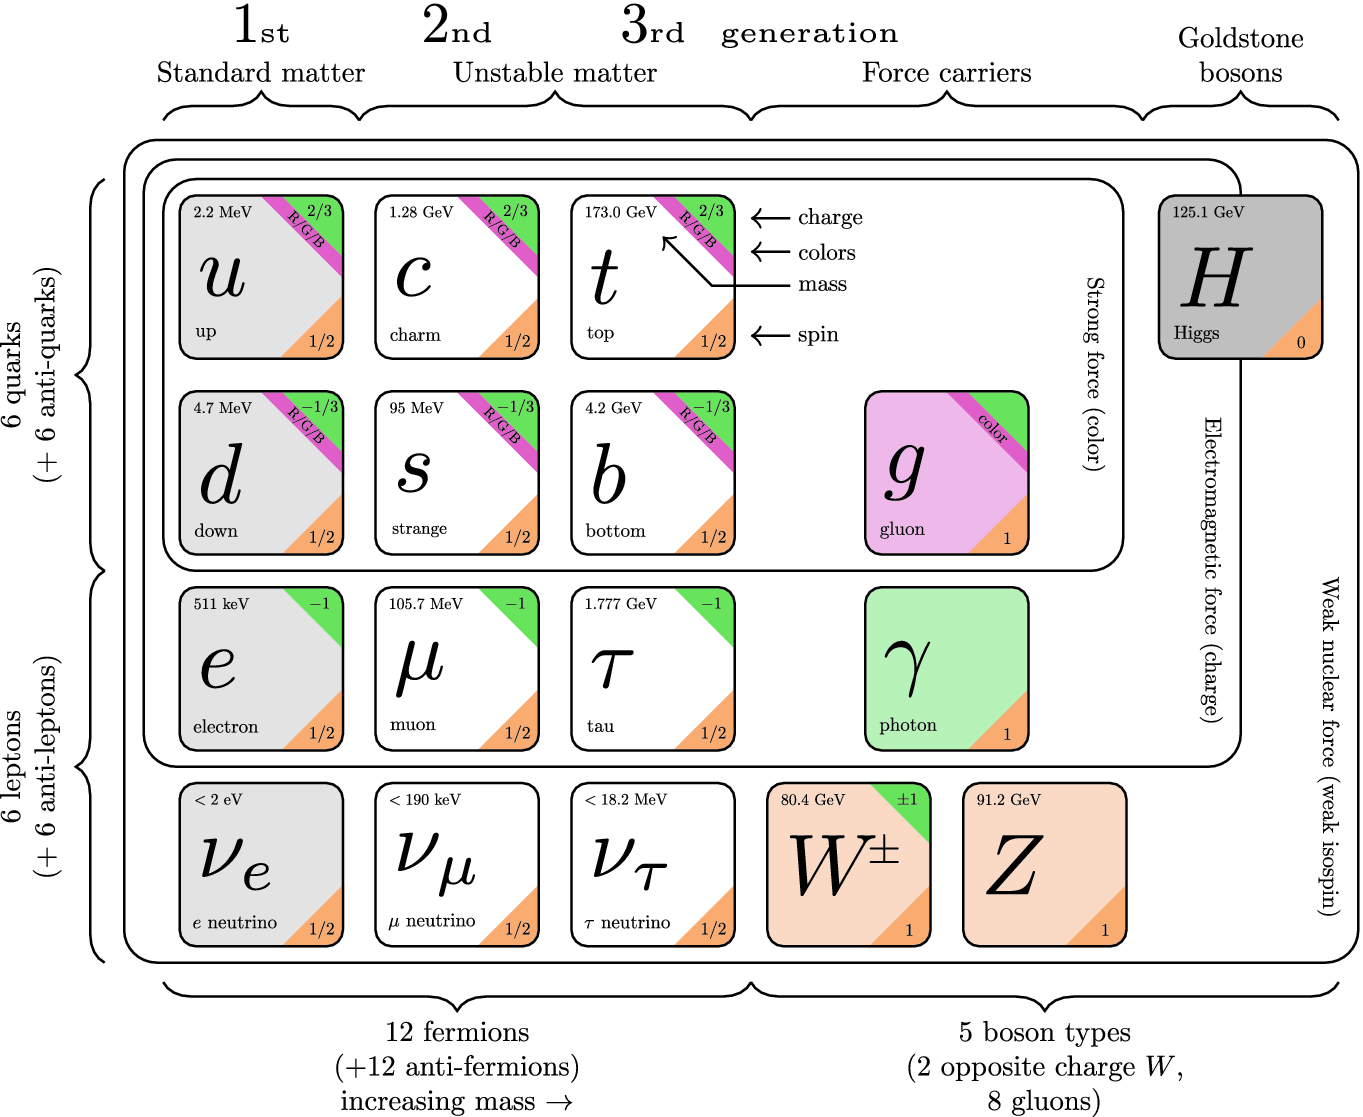
\includegraphics[width=8cm, height=6cm]{figs/SMFermions.png}
\caption{Representation of the 12 fermions of the Standard Model \cite{SMFermions} along with the main force carriers and the Higgs boson, discovered in 2012 and completing this model.}
\label{figure:SMFermions}
\end{center}
\end{figure}

Muons $\mu^{-}$ \cite{PDGMuons} are therefore fundamental particles having a negative charge and quite similar in nature to electrons, even though they have a quite high mass (200 times larger than the electron), which implies that their are not stable particles: they have a lifetime of approximately 2.2$\mu$s, and typically decay into an electron and a pair of neutrinos. However, this lifetime is actually quite long with respect to other fundamental particles and muons are on average able to travel more than 700 meters, allowing us to consider them to be stable particles in many processes, such as the one presented in this work. Muons also have a relatively small interaction cross-section with ordinary matter, even though they do interact with baryonic matter by several processes described in Section~\ref{sec:interactions}.

\section{Cosmic rays} \label{sec:cosmicRays}

Being unstable by nature, once produced, muons decay almost instantly by a weak process into an electron and a pair of neutrinos. However, it is possible to observe them in nature, since they are continually produced, mainly thanks to cosmic rays \cite{cosmicPDG}, constant flux of high energy particles (mostly protons and atomic nuclei) coming mostly from supernovae explosions and AGN emissions and reaching the Earth every day. Indeed, as they impact our atmosphere, these particles start a chain reaction, as shown in Figure~\ref{figure:cosmic}: first of all, several neutral and charged pions are produced, decaying themselves into a pair of photons (and, later on, electron and positron pairs) and muons, respectively.

\begin{figure}[htbp]
\begin{center}
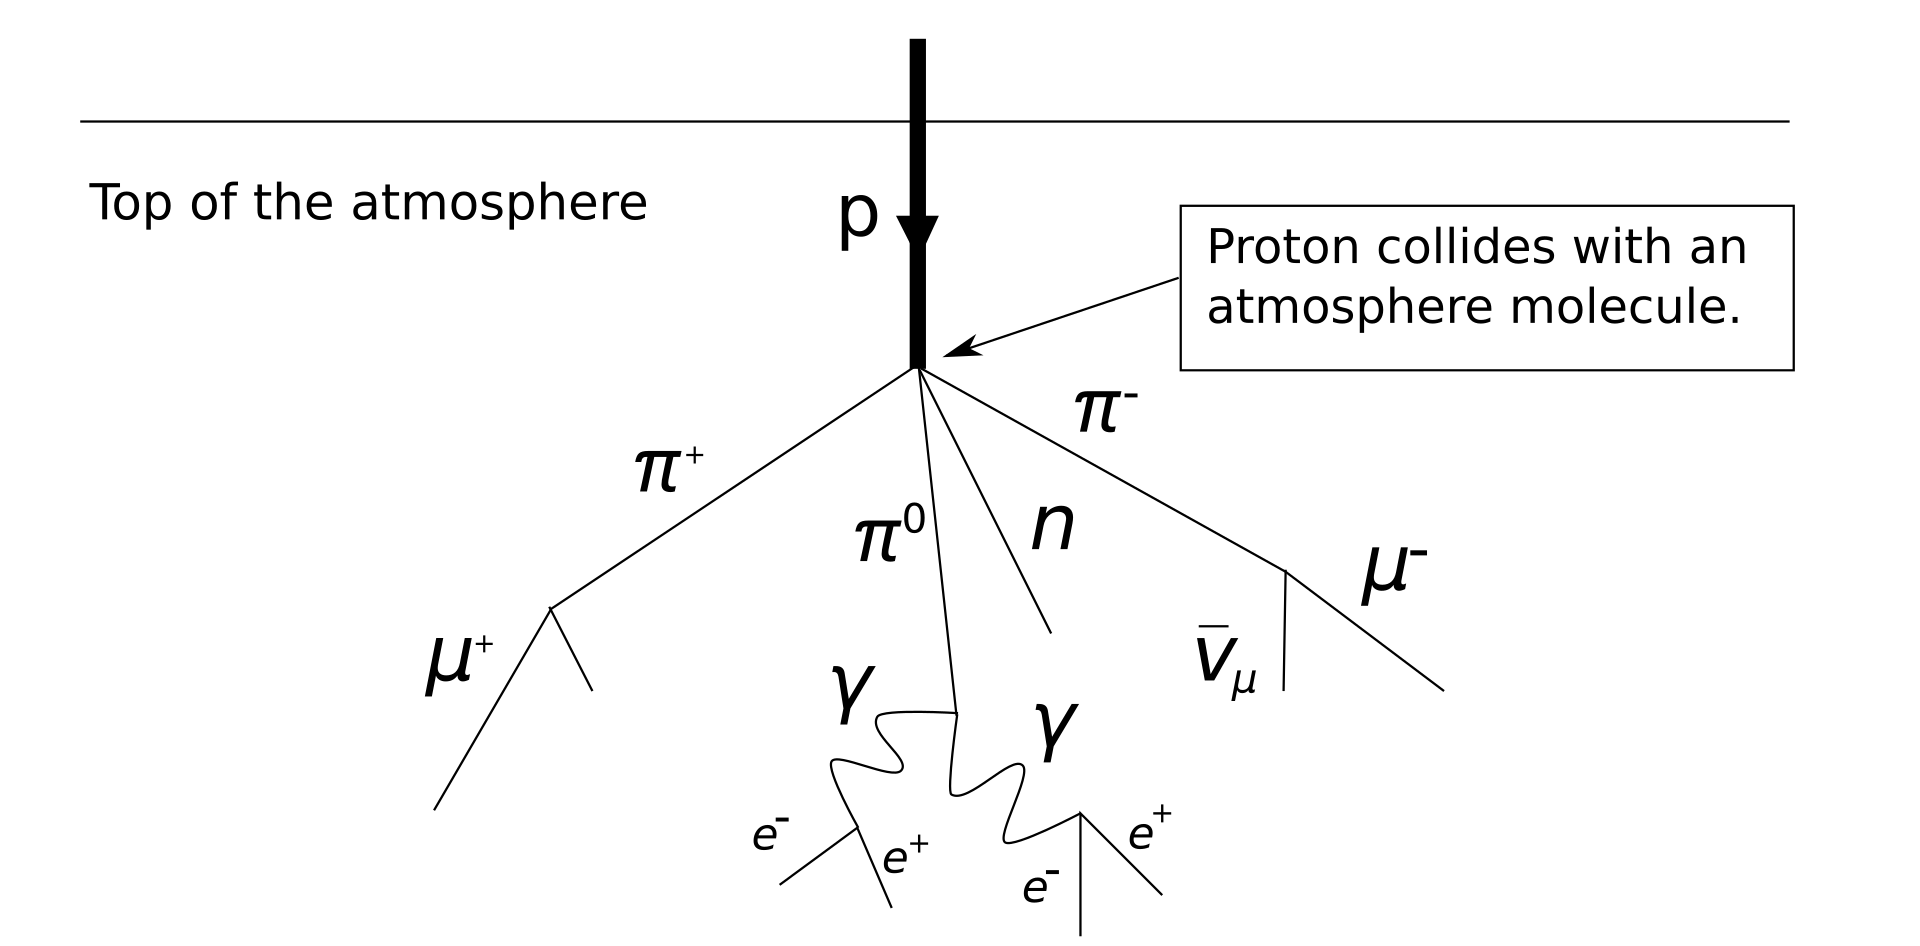
\includegraphics[width=11cm, height=6cm]{figs/cosmic.png}
\caption{Typical chain of decays induced by highly energetic cosmic rays when reaching the Earth's atmosphere.}
\label{figure:cosmic}
\end{center}
\end{figure}

Muons are the most abundant charged particles produced by these processes actually reaching the sea level, as shown in Figure~\ref{figure:cosmicAbundance}. Even though they are unstable and have a limited lifetime, around 0.06\% of muons produced by such processes indeed do manage to reach the sea level thanks to the temporal distorsion induced by their high energy and relativistic speed. As a rule of thumb, one can expect to observe 10.000 muons per square meter and per minute at the sea level.

\begin{figure}[htbp]
\begin{center}
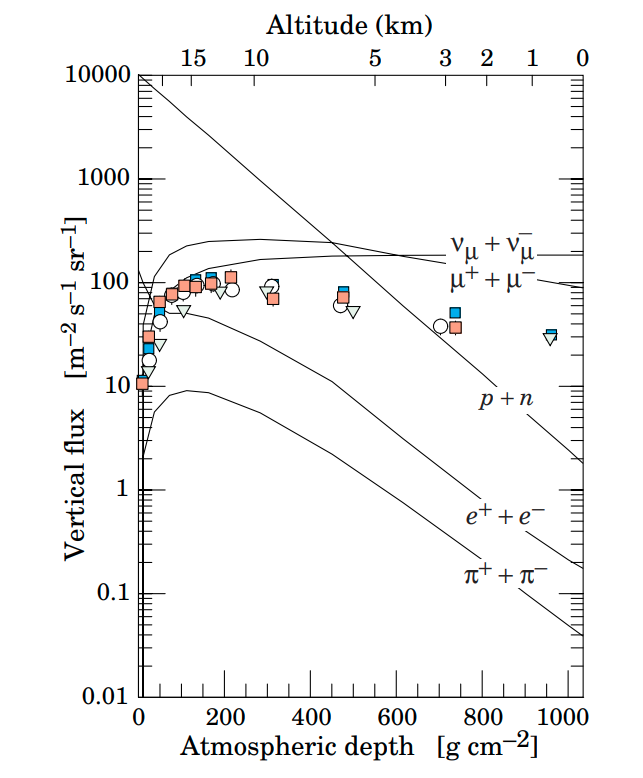
\includegraphics[width=8cm, height=9cm]{figs/cosmicMuons.png}
\caption{Abundance of particles observed at the sea level, due to cosmic rays \cite{cosmicPDG}.}
\label{figure:cosmicAbundance}
\end{center}
\end{figure}

Muons were actually discovered thanks to cosmic rays in 1936 \cite{muonDiscovery}.

\section{Muons interaction with matter} \label{sec:interactions}

Muons typically interact with ordinary matter through two main processes: ionization and multiple scattering, both resulting in different effects on the incident particle.

\subsection{Ionization process}

The most frequent interaction process of cosmic muons is through \textbf{ionization}, when the incident muon is giving some of its energy to the electrons of the absorber. This process is described by the Bethe-Bloch formula, shown in Equation~\ref{eq:BB}, and describing the average loss of energy over a distance $\frac{dE}{dx}$ of material, depending on several parameters, such as the charge number of incident particle $z$, the atomic mass and charge of absorber $A$ and $Z$, the relativistic factors $\beta$ and $\gamma$, the maximum possible energy transfer to an electron in a single collision $W_{\text{max}}$ and the mean excitation energy $I$.

\begin{equation}
\label{eq:BB}
- \Bigl \langle \frac{dE}{dx} \Bigr \rangle = K z^2 \frac{Z}{A} \frac{1}{\beta^2} \left [\frac{1}{2} \ln \left (\frac{2 m_e c^2 \beta^2 \gamma^2 W_{\text{max}}}{I^2} - \beta^2 - \frac{\delta(\beta \gamma)}{2} \right ) \right ]
\end{equation}

This previous equation gives an accuracy of a few percent in the range $0.1 < \beta < 1000$ and we can easily see that the quantity of energy lost by in a muon when traversing any given medium actually depends on the energy of the incident muon, as shown in Figure~\ref{figure:BB}.

\begin{figure}[htbp]
\begin{center}
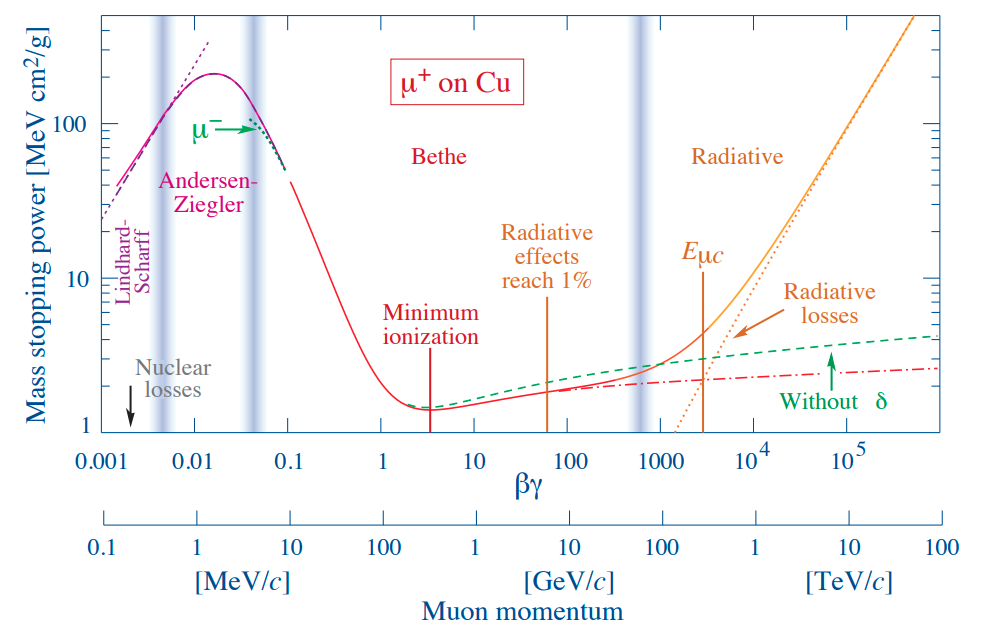
\includegraphics[width=12cm, height=8cm]{figs/BB.png}
\caption{Average energy lost a muon due to ionization depending on its momentum \cite{PDGMuons}.}
\label{figure:BB}
\end{center}
\end{figure}

In practical cases, most relativistic particles, such as muons coming from cosmic rays, have mean energy loss rates actually close to the minimum. They are usually called for this reason \textit{minimum ionizing particles} or MIPs.

\subsection{Multiple scattering process}

Muons also interact with matter through another process, called \textbf{multiple scattering}. Since muons have a negative electric charge, by getting close to the nuclei of the absorber, they are suffering from Coulomb scattering. Given the high number of nuclei in matter, this process is repeated many times, deflecting each time the muon by a small angle in a stochastic way, meaning that there is no way of calculating this deviation exactly, but only using probabilities and the so-called theory of Moli�re \cite{Moliere}, shown in Equation~\ref{eq:Moliere}, where $\theta_0$ is the expected angle of deviation shown in Figure~\ref{figure:Moliere}, $p$ is the momentum of the incident particle and $X_0$ is the radiation length, defined as the characteristic amount of matter traversed by the incident particle for a particular interaction.

\begin{equation}
\label{eq:Moliere}
\theta_0 = \frac{13.6 \text{ MeV}}{\beta c p} z \sqrt{\frac{x}{X_0}} \left [1 + 0.038 \ln \left (\frac{x z^2}{X_0 \beta^2} \right ) \right ]
\end{equation}

This formula is expected to be valid for distances up to $\sim 100 X_0$, giving an error smaller than 11\% \cite{PDGMuons}. Corrections do exist though in order to get slightly better results, but this theory is precise enough for our needs, given the experimental conditions considered in this work.

\begin{figure}[htbp]
\begin{center}
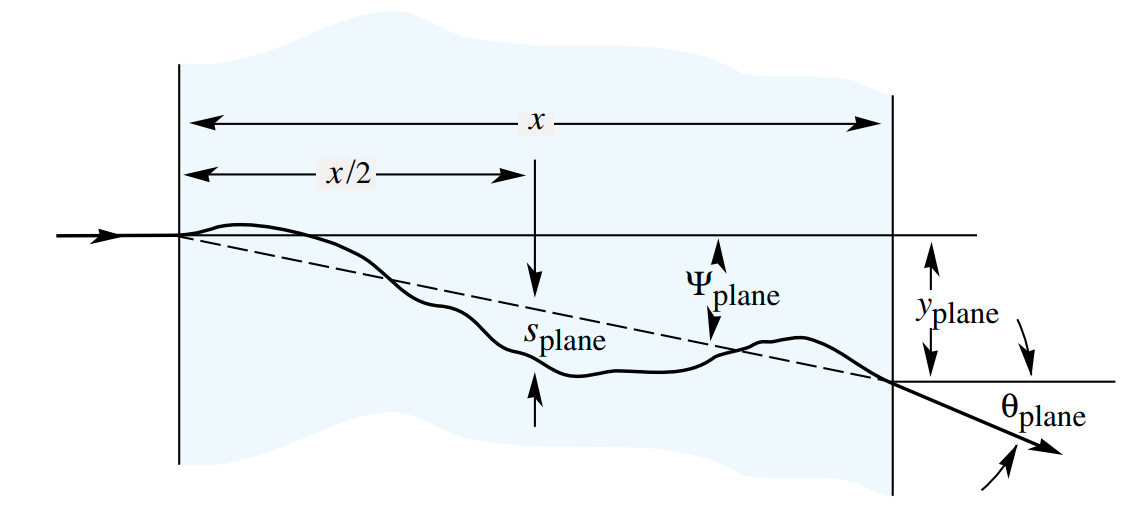
\includegraphics[width=12cm, height=5.2cm]{figs/moliere.png}
\caption{Schematic representation of the deviation induced by an absorber to an incident muon because of the multiple scattering effect \cite{PDGMuons}.}
\label{figure:Moliere}
\end{center}
\end{figure}

\section{Muon tomography} \label{sec:tomography}

Given Moli�re's theory, it is obvious to see that, instead of \textit{calculating} the deviation of a muon crossing a given material, we can instead try and \textit{measure} it, by inversing the two previous relations. Since this deviation depends on several parameters related to the absorber itself, such as its width and radiation length $X_0$, we can in this case actually infer such parameters experimentally and determine the properties of the medium crossed by cosmic muons. This is the so-called muon tomography, or \textbf{muography}, taking advantage of the interaction of muons with matter to use it in practice.

Muography is therefore a non-destructive imaging technique producing a density map of the inside of an object by measuring a flux of muons. Such method presents many different advantages over other imaging techniques such as X-rays, since it actually uses natural cosmic rays to make the measurements, being therefore completely safe. Additionally, muons interact lightly with matter, meaning that they typically have high penetrating capabilities and can therefore probe even large and/or dense objects. Muography can in this sense be applied to many different fields: it has for example even been used in 1970 in order to try and find hidden cavities of pyramids in Egypt \cite{Egypt} and can also be used in vulcanology, to determine whether a pocket inside of a volcano is empty or full of lava, among many other practical applications.

Such imaging techniques can be divided into two categories:
\begin{itemize}
\item \textbf{Absorption muography}. In this case, the observed muon flux in a given direction is compared to what is expected from cosmic rays, trying to determine the inner structure of the absorber as discrepancies between these two values. Only one detector is needed in this case, making this technique useful mostly to study large objects, even though the time to make a single measurement can last up to a few months.
\item \textbf{Scattering muography}. On the other hand, the multiple scattering of muons can be used, by placing one detector on each side of the object being studied to determine the deviation of the flux of incoming muons. The denser the material put in between, the larger the observed deviation will be, as shown in Equation~\ref{eq:Moliere}. This technique is mostly used to study smaller objects and is able to make quick measurements.
\end{itemize}

In this particular work, scattering muography is being applied to industry in order to try and determine the degradation of the interior of industrial equipment, as we will now see.

\section{Experimental setup} \label{sec:setup}

\subsection{Muon detectors} \label{sec:muonDetectors}

If we want to work with cosmic muons, we need to be able to build some detectors able to spot them and give us back useful data, such as their energy and/or incident direction. Many different technologies exist nowadays in order to detect muons, even though in this particular case, the typical \textbf{multi-wire proportional chambers} have been used.

Invented at CERN in 1968, these detectors use an array of high-voltage wires (playing the role of the anode), running through a chamber filled with gas and whose walls are typically grounded (the cathode), as shown in Figure~\ref{fig:wireChambers}. Such an experimental setup therefore creates an electric field inside of the chamber, that needs to be made as large and uniform as possible.

\begin{figure}[htbp]
\begin{center}
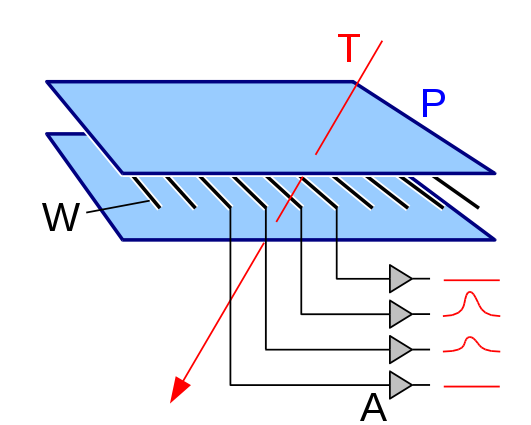
\includegraphics[width=7cm, height=5.2cm]{figs/wireChambers.png}
\caption{Schematic representation of a wire chamber muon detector.}
\label{fig:wireChambers}
\end{center}
\end{figure}

When a charged particle such as a muon crosses this chamber, it will ionize the gas of the chamber and leave small electric charges along its path which will start to drift until reaching one of the wire. This drift induces an electric signal proportional to the ionisation effect in the different wires surrounding the particle path, and the combination of all the signals collected is able to give information regarding the actual path followed by the incoming particle.	

Several properties are extremely important when designing a detector:
\begin{itemize}
\item First of all, the \textbf{spatial resolution}, the precision by which we can tell the position of the muon, should be ideally as small as possible, depending on the actual problem faced.
\item The \textbf{efficiency} is also an important parameter, since we want to be able to detect as many muons as possible, to make the measurement faster and more precise.
\item Finally, we typically want the detector to be large enough to avoid any \textbf{acceptance} issues.
\end{itemize}

\subsection{Working setup} \label{sec:ourSetup}

For this particular work, four muon chambers of 1 meter by 1 meter have been build using these principles, as shown in Figure~\ref{fig:setup}. As we can see, more than 200 wires connected to the high voltage and made out of gold and tungsten have been placed every 4mm in two different planes rotated by 90 degrees, to measure the $x$ and $y$ postion of cosmic muons. 

These chambers, filled while a mixture of Argon and CO$_2$, are then setup in pairs above and below the object being studied, in order to determine the position and the direction of the incoming and outgoing cosmic muon. This setup allows to measure with a good spatial resolution the deviation of muons, to determine as precisely as possible the properties of the object put in between both detectors.

\begin{figure}[htbp]
\centering
\begin{minipage}[b]{.59\textwidth}
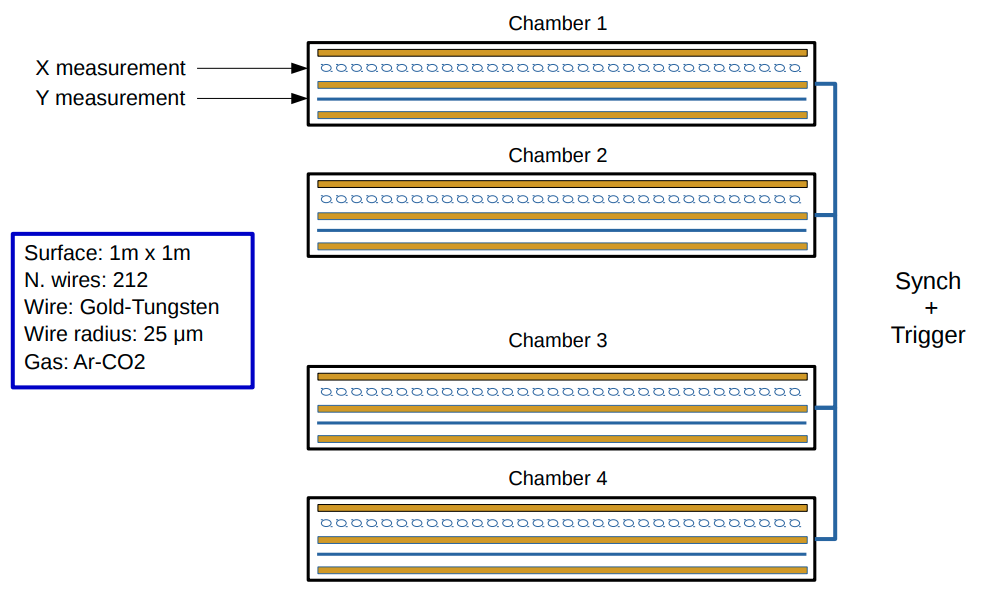
\includegraphics[width=9cm, height=6cm]{figs/muonChambers.png}
\end{minipage}\hfill
\begin{minipage}[b]{.39\textwidth}
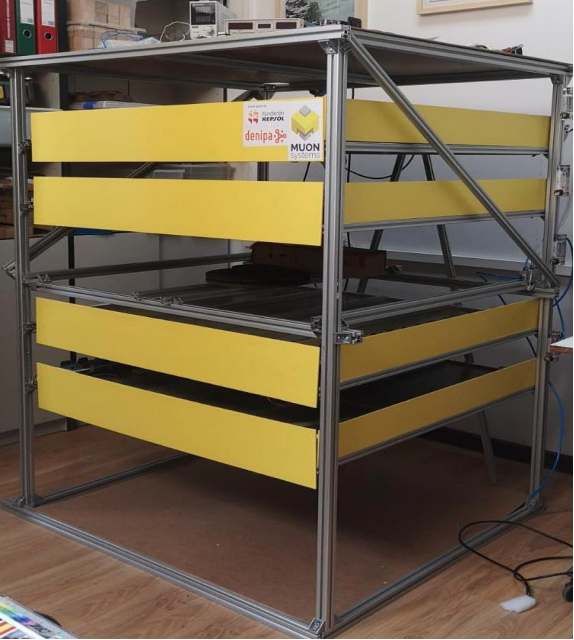
\includegraphics[width=6cm, height=6cm]{figs/muonChambersPhoto.png}
\end{minipage} \hfill
\caption{Actual working setup used for this work, with two multi-wires muon chambers of 1m$^2$ placed on each side of the object being studied.}
\label{fig:setup}
\end{figure}

\subsection{Data flow} \label{sec:dataFlow}

Once collected, the data needs to be pass through several differents in order to convert electric signals into files that can be processed, as shown on Figure~\ref{fig:dataFlow}. As we can see, the data follows a different path depending on its nature, if it has been collected by the detector or if we are considering Monte-Carlo simulations that will be described in details in the next Chapter. The stream of data is collected by a simple USB, and then sent to a DAQ/DQM system and to an unpacker, which takes into account the detector gemetry and translates into a physical position the information received from the DAQ, typically only telling that a certain wire has been activated.

Both streams then join at the 1D histogram format level, gathering a collection of all the hits measured for every event. All these hits are then processed and reconstructed into two trajectories, one above and one below the object, using advanced techniques that will also be described in next Chapter. Finally, 4D segments are made available from this reconstruction process, having the position and direction information needed, from which the actual analysis can take place.

\begin{figure}[htbp]
\begin{center}
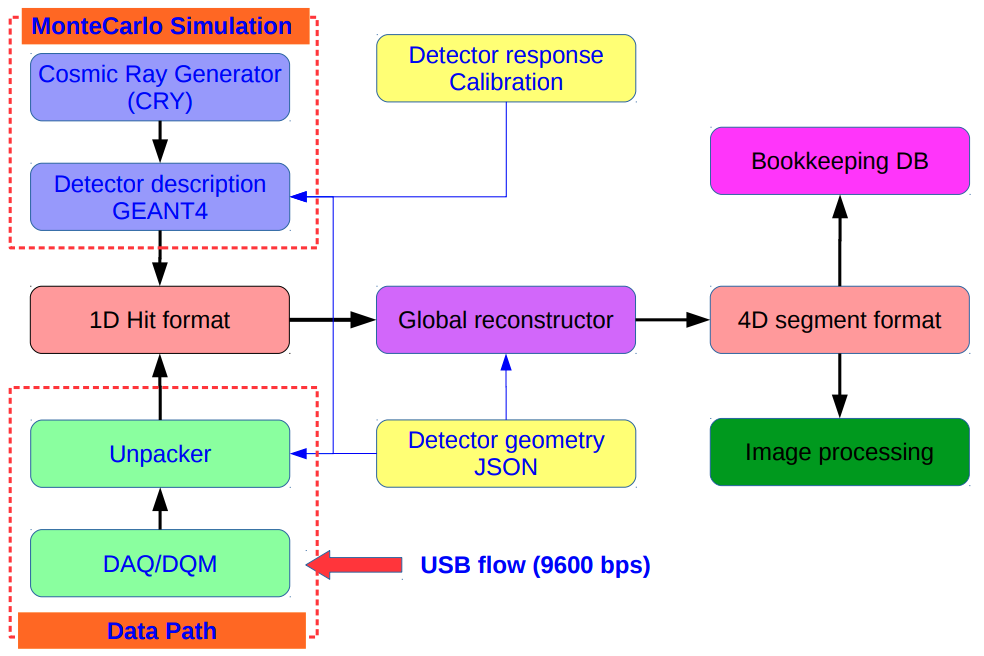
\includegraphics[width=8.5cm, height=6cm]{figs/dataFlow.png}
\caption{Schematic representation of the detector data flow.}
\label{fig:dataFlow}
\end{center}
\end{figure}



























\chapter{Statistical parameters}

The general objective of this work is to find a way to determine the geometry of an eventual object placed between the two muon detectors by measuring the deviation affecting incident cosmic muons, a typical non-deterministic process which therefore needs to be adressed using advanced statistical parameters ans methods, such as probability and kernal density functions (Sections~\ref{sec:PDF} and~\ref{sec:KDF}), Monte-Carlo simulations (Section~\ref{sec:MC}), p-values (Section~\ref{sec:pValues}) and likelihood function (Section~\ref{sec:Likelihood}).

\section{Probability density functions} \label{sec:PDF}

The probability density functions, or PDFs, are statistical expressions defining probability distributions representing the likelihood of any given outcome. They are typically represented as curves in the two dimentional space (x, y), as shown in Figure~\ref{fig:PDF}, in which the total area below the curve in an interval is equal to the probability of a discrete random variable occurring. 

\begin{figure}[htbp]
\begin{center}
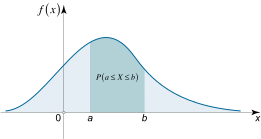
\includegraphics[width=12cm, height=5.4cm]{figs/PDF.png}
\caption{Schematic representation of a random PDF \cite{PDF}.}
\label{fig:PDF}
\end{center}
\end{figure}

Gaussian distributions are in this sense probability density functions having a particular expression defined in Equation~\ref{eq:gauss}, where $\sigma$ is the so-called \textbf{standard deviation} of the distribution, representing its width: a low $\sigma$ indicates that the values of the distribution tend to be close to its mean value $\mu$, while a high $\sigma$ indicates that the values are spread out over a wider range.

\begin{equation}
\label{eq:gauss}
f(x) = \frac{1}{\sqrt{2 \pi} \sigma} e^{-\frac{1}{2} \left (\frac{x - \mu}{\sigma} \right )^2}
\end{equation}

These definitions are important because we already know that the multiple scattering process which affects the incident cosmic muons is a stochastic process: this means that two muons having similar kinematics can leave the detector with very different output directions and positions, whose actual distribution can be approximated by a gaussian function for small deviation angles (at larger angles, the distribution is behaving like Rutherford scattering, with slightly larger tails). 

The standard deviation of the distribution of such output paraemeters is actually highly dependant on the geometrical parameters $\theta_i$ of the eventual object put between the two detectors, as we saw in Equation ~\ref{eq:Moliere}. Indeed, the mean deviation observed is expected to depend on the number of radiation lengths crossed, typically much higher when a muon crosses denser objects, such as a steel pipe, as shown in Figure~\ref{fig:deviation}. This means that in first approximation, the tichker the object investigated is, the higher the expected deviation will be and this simple observation will actually be used as the driving process of the statistical study performed in this work.

\begin{figure}[htbp]
\centering
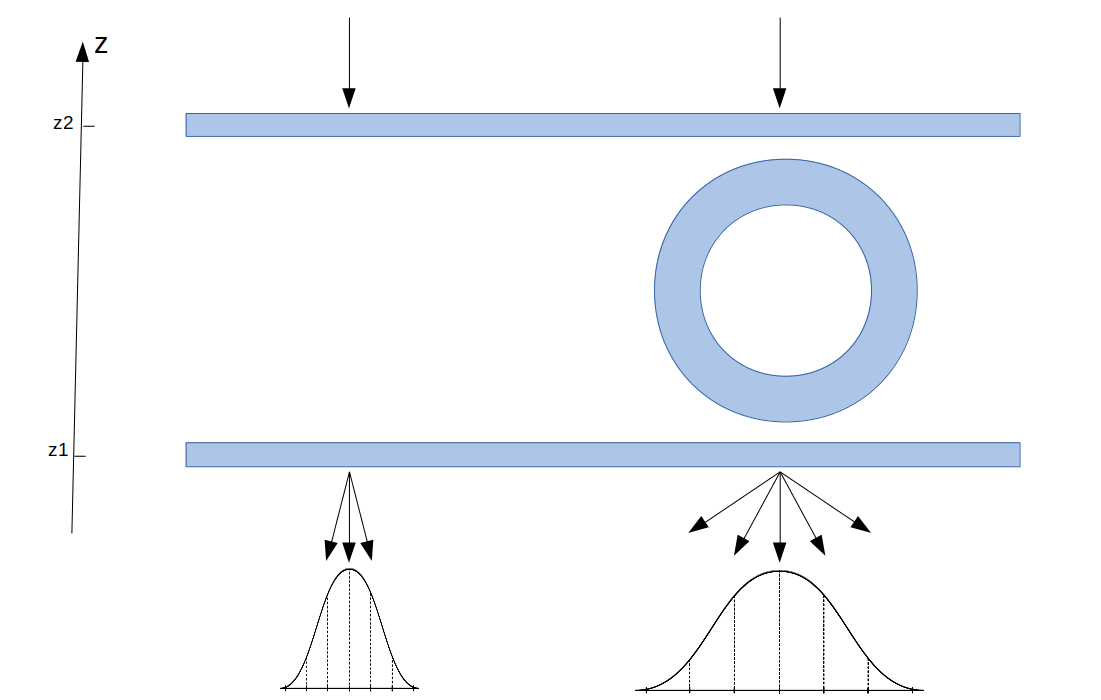
\includegraphics[width=12cm, height=7cm]{figs/pdfs.png}
\caption{Schematic representation of the deviation expected for an incoming muon and PDFs associated without (on the left) and with (on the right) an object placed between the detectors.}
\label{fig:deviation}
\end{figure}

\section{Monte-Carlo simulations} \label{sec:MC}

Monte-Carlo simulations are algorithms developped in order to compute approximate numerical values to stochastical problems using random processes and advanced probabilistic techniques. In this particular case, such computation methods apply extremely well since, by being a stochastical process, the actual probability density function associated to a given geometry cannot be computed analytically (and if we were able to do it, a simple gradiant descent method would be enough to solve this problem and find the optimal parameters $\theta_i$ of the object). 

The only way available to actually estimate these parameters is by using thousands of Monte-Carlo simulated toys, simulating thousands of different incident muons for different geometries. The principle is simple: for each incident muon measured, a large number $N$ of Monte-Carlo simulations will be performed, propagating the muon using an algorithm described in Chapter~\ref{chapter:algorithm} until reaching the lower detector. Repeating this experiment over and over again always gives different results, giving us the opportunity to build the expected PDF for a given object geometry and for the incident muon that has been measured and that will be used later on.

At the end of the day, the main objective of this process is to be able to estimate the probability of observing a certain deviation given an object geometry and the input trajectory of the muon, $P$(deviation$|$input) in simulation. Then, this process will be reversed using actual data in order to try and obtain the geometry of the object from the actual measurement of the input and output muon trajectories and positions, using a likelihood minimization method.

\section{p-values} \label{sec:pValues}

So far, we developed a technique allowing us to reconstruct the expected probability density function for a given incident muon using Monte-Carlo techniques. However, we still need a way to estimate the goodness of the actual measurement with this simulated PDF: this is where the so-called \textbf{p-values} enter, a key ingredient for this work since they allow to relate the two main parts of the problem: the simulations performed and the actual data collected.

Probability values, or p-values, are based on the concept of \textbf{null hypothesis $H_0$}, a general statement or default position telling that there is no actual relationship between two measured phenomena and assumed to be true until an evidence indicates otherwise. This hypothesis is then typically opposed to the \textbf{alternative hypothesis $H$}, usually more interesting by being the interesting hypothesis of the experiment being performed. The main goal is to compare the data with both hypotheses: if the data is consistent with $H_0$, then the null hypothesis can simply not be rejected. However, we can reject $H_0$ (and therefore accept $H$, its exact opposite) if the data collected is significantly unlikely to have occurred if the null hypothesis were to be true, according to a \textbf{confidence level} previously defined.

From these definitions, a p-value is then defined as the probability for a variable to be observed equal or more extreme (lower or higher, depending on the cases) than the actual value $x$ observed under the null hypothesis. This definition, can be represented in a schematic way in Figure~\ref{fig:pvalue}.

\begin{figure}[htbp]
\centering
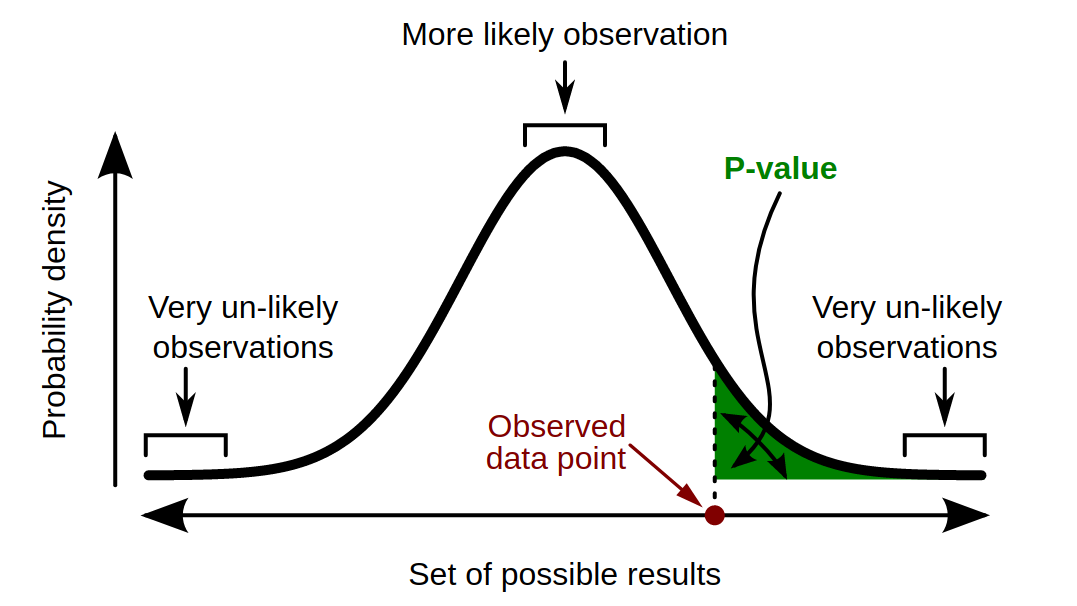
\includegraphics[width=13cm, height=7cm]{figs/pvalue.png}
\caption{Schematic representation of the statistical concept of p-value.}
\label{fig:pvalue}
\end{figure}

In general, a smaller the p-value tells us that the hypothesis under consideration may not adequately explain the observation, leading to a higher statistical significance. At the end of the day, the null hypothesis is rejected if the p-value obtained is smaller than a previously defined, arbitrary and fixed threshold $\alpha$, the \textbf{level of significance} of the experiment. This parameter can take a large range of values, typically ranging from 0.05 to 0.001.

In this work, the p-value will then allow us to compare a single data measurement with the probability density functions obtained from Monte-Carlo and quantify the probability that such muon was actually observed for a given object geometry. This value will then be feeded to a likelihood function, as explained in Section~\ref{sec:Likelihood}.

\section{Kernel density functions} \label{sec:KDF}

In statistics, the kernel density estimation is a method allowing to estimate the density probability of a random variable. The objective of this method is to make inferrence regarding the data in order to try and smooth the probability density function obtained experimentally, as shown in Figure~\ref{fig:KGR}.

\begin{figure}[htbp]
\centering
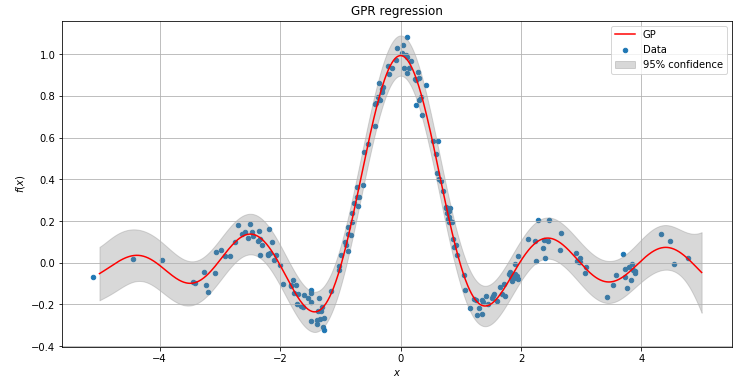
\includegraphics[width=13cm, height=7cm]{figs/GPR.png}
\caption{Academic example of a gaussian regression applied to a noisy and finite set of data points.}
\label{fig:KGR}
\end{figure}

Mathematically, the objective is then to build a continous function $\hat{f}_h(x)$ defined in Equation~\ref{eq:KDF} from a finite set of data samples $\bm x$, distributed along an unknown density function $f$, and where $K$ is the so-called \textbf{kernel} and $h$ is the \textbf{bandwidth} or \textbf{smoothing parameter} of the estimation.

\begin{equation}
\label{eq:KDF}
\hat{f}_h(x) = \frac{1}{nh} \sum_{i=1}^{n} K \left (\frac{x-x_i}{h} \right )
\end{equation}

In the previous equation the kernel $K$ is a non-negative function defined depending on the problem, as the "building block" of the final function that needs to be estimated: indeed, as we can see, the function $\hat{f}_h(x)$ will be given as a simple sum of kernels. In most of the problems, including this work, a standard gaussian kernel is used, taking the shape shown in Equation~\ref{eq:kernel}.

\begin{equation}
\label{eq:kernel}
K(x) = \frac{1}{\sqrt{2 \pi}} e^{-\frac{1}{2} x^2}
\end{equation}

In this particular case, this method allows us to construct continous functions and recover for the eventual low statistics and possibles holes in the bi-dimentional histograms for the position and direction of the muons obtained in $x$ and $y$, following the method that will be described in Chapter~\ref{chapter:algorithm}.

\section{Likelihood} \label{sec:Likelihood}

So far, we have been able to generate thousands of different Monte-Carlo experiments for a given muon and for a given object geometry, but we still need to find a way to reverse this process to estimate the geometry of the object from a given measurement. 

This is where the likelihood becomes useful, defined as a function that measures the goodness of a fit with respect to a sample of data, for several unknown parameters of a mathematical model. In general, this function can be defined in Equation~\ref{eq:likelihood}, where $\bm \theta = $\{$\theta_1, ..., \theta_i$\} are the parameters of the model and $x$ is the actual measurement of a random variable $X$ following a density function $f$.

\begin{equation}
\label{eq:likelihood}
\mathcal{L}(\bm \theta | x) = f_{\bm \theta}(x) = P(X = x | \bm \theta)
\end{equation}

It is important to note at this point that the likelihood is a function of the parameters $\bm \theta$ but not a probability density function itself. Additionally, it should in general not be confused with the probability $p(\bm \theta | x)$ since it is equal to the probability of observing a given outcome $x$ when the true values of the parameters are $\bm \theta$: this means that the likelihood is equal to a probability density over the outcome $x$, not over the parameters $\bm \theta$.

To understand this concept better, the simple example of an unfair coin toss can be considered, where the fairness of the coin is the parameter of the model, represented by the probability of obtaining head $p_H$ and taking values between 0 and 1 (for a regular coin, $p_H = 0.5$). The likelihood is then defined from a given observation, such as obtaining two heads in a row $HHT$ in the following way:

\begin{equation}
\label{eq:likelihoodEx}
\mathcal{L}(p_H | HHT) = P(HHT | p_H) = P(H | p_H) \cdot P(H | p_H) \cdot P(T | (1-p_H))
\end{equation}

For each value of $p_H$, the value of the likelihood can then be computed and ultimately plotted, as shown in Figure~\ref{fig:likelihoodEx}, showing a minimum value for a particular value of $p_H$.

\begin{figure}[htbp]
\centering
\begin{minipage}[b]{.49\textwidth}
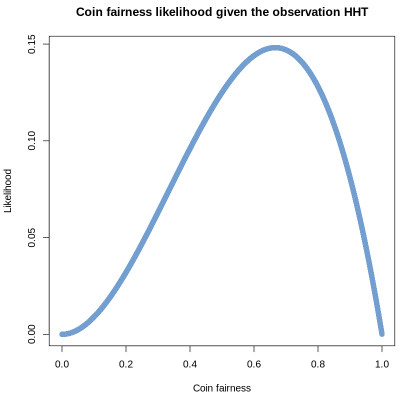
\includegraphics[width=7cm, height=6cm]{figs/likelihood.png}
\end{minipage}\hfill
\begin{minipage}[b]{.49\textwidth}
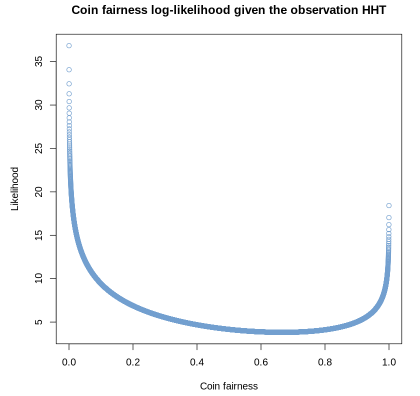
\includegraphics[width=7cm, height=6cm]{figs/loglikelihood.png}
\end{minipage} \hfill
\caption{Likelihood (on the left) and log-likelihood (on the right) obtained for our particular example of the fairness of a coin given the observation $HHT$.}
\label{fig:likelihoodEx}
\end{figure}

The likelihood is in this sense interesting because it can be described as a hypersurface whose peak gives the optimal set of parameters maximizing the probability of drawing the actual sample measured. Often, the \textbf{log-likelihood} $l(\bm \theta | x) = -2 \log(\mathcal{L}(\bm \theta | x))$ is actually used instead, being a bit more convenient to deal with the special part concavity plays in the maximization process. Given the properties of the logarithm, maximizing the likelihood is equivalent to minimizing this particular log-likelihood.

Another important property of the likelihood that will be used extensively and already assumed in the previous example is the fact that, for two independant measurements, the likelihood of both measurements is equal to the product of both likelihoods independantly computed for each event.

In this work, a likelihood function will be obtained as the product of the thousands of muons collected, but for a fixed geometry of the object. A minimization method will then be performed in order to try and minimize the value obtained by trying out different parameters $\bm \theta$, until finding the optimal set of parameters able to describe best the object put in between the detectors.












%In this work, measurements of cosmic muons are taken for a relatively long period of time to accumulate statistics. Each event recorded is independent from the previous one by nature, and our goal is to estimate from the ingredients previously defined the actual geometry of the object placed between the detectors, defined from a set of parameters $\bm \theta$.


















\chapter{The algorithm} \label{chapter:algorithm}

Muons described by 6 parameters.

\chapter{Results obtained}

\chapter{Conclusions}

%\begin{appendices}
  
%\chapter{Appendix1}
  
%\end{appendices}

\addcontentsline{toc}{chapter}{Bibliography}

\begin{thebibliography}{1}

\bibitem{SM}
\href{https://arxiv.org/abs/hep-ph/0510281}{G. Altarelli,
"The Standard Model of Particle Physics",
CERN-PH-TH/2005-206, 2005}

\bibitem{topQuark} 
\href{https://arxiv.org/abs/hep-ex/9503003}{D0 Collaboration,
"Observation of the Top Quark",
Phys.Rev.Lett.74:2632-2637, 1995}

\bibitem{tauNeutrino} 
\href{https://arxiv.org/abs/hep-ex/0012035}{DONUT Collaboration, 
"Observation of Tau Neutrino Interactions",
Phys.Lett.B504:218-224, 2001}

\bibitem{HiggsDiscovery1} 
\href{https://arxiv.org/abs/1207.7235}{S. Chatrchyan et al.,
"Observation of a new boson at a mass of 125 GeV with the CMS experiment at the LHC",
Phys.Lett.B716:30-61, 2012 [arXiv: 1207.7235]
}

\bibitem{HiggsDiscovery2} 
\href{https://arxiv.org/abs/1207.7214}{G. Aad et al.,
"Observation of a new particle in the search for the Standard Model Higgs boson with the ATLAS detector at the LHC", 
Phys.Lett.B716:1-29, 2012 [arXiv: 1207.7214]}

\bibitem{CMS}
\href{http://inspirehep.net/record/796887/}{CMS Collaboration,
"The CMS Experiment at the CERN LHC",
JINST 3 S08004, 2008}

\bibitem{ATLAS}
\href{http://inspirehep.net/record/796888/}{ATLAS Collaboration,
"The ATLAS Experiment at the CERN Large Hadron Collider",
JINST 3 S08003, 2008}

\bibitem{SMFermions}
\href{https://link.springer.com/chapter/10.1007/978-3-030-24370-8_2#citeas}{S. Manzoni, 
"The Standard Model and the Higgs Boson",
Physics with Photons Using the ATLAS Run 2 Data, Springer Theses, 2019
}

\bibitem{PDGMuons}
\href{http://pdg.lbl.gov/2018/listings/rpp2018-list-muon.pdf}{
"Muon", Particle Data Group, 2018}

\bibitem{cosmicPDG}
\href{http://pdg.lbl.gov/2017/reviews/rpp2017-rev-cosmic-rays.pdf}{
"Cosmic rays", Particle Data Group, 2017}

\bibitem{muonDiscovery}
\href{http://web.ihep.su/dbserv/compas/src/neddermeyer37/eng.pdf}{S.H. Neddermeyer and C.D. Anderson,
"Note on the Nature of Cosmic-Ray Particles", 
Physical Review Vol. 51, 1936}

\bibitem{Moliere}
\href{https://journals.aps.org/pr/abstract/10.1103/PhysRev.89.1256}{H.A. Bethe,
"Moli�re's Theory of Multiple Scattering", 
Physical Review Vol. 89, 1953}

\bibitem{Egypt}
\href{https://ui.adsabs.harvard.edu/abs/1970Sci...167..832A/abstract}{L. Alvarez et all.,
"Search for Hidden Chambers in the Pyramid", 
Science, Volume 167, Issue 3919, 1970}

\bibitem{PDF}
\href{https://www.math24.net/probability-density-function/}{Math24, "Probability Density Function", as seen in May 2020}

\end{thebibliography}

\end{document}
